%-------------------------------------------------------------------------------
% RESULTS
%-------------------------------------------------------------------------------

\section{Results} \label{sec:res}

\subsection{Outline of Bifurcation Diagram}

The primary objective of this project was to reproduce the bifurcation diagram
presented in figure \ref{fig:bif_diag_chen} of \citet{chen2013}. The resulting
bifurcation diagram of the regularized version is depicted in figure
\ref{fig:bif_diag}, and a table is provided, listing the bifurcations that
occurred along with their corresponding critical Reynolds numbers. As
mentioned, only a square cavity is considered for this study, and no aspect
ratios have been varied.

The critical Reynolds numbers reported were determined by linearly
interpolating the eigenvalues between two states of the pseudo-arclength
continuation algorithm where the eigenvalue crosses the imaginary axis in the
complex plane. When eigenvalues are only touching the real line (i.e., no
crossing), the Reynolds number with the smallest eigenvalue evaluated has been
reported. The reported results are rounded to three significant digits.

\begin{table}[h!]
  \centering
  \caption{List of bifurcations encountered and the critical $\Rey$ at which they
    occur}
  \label{tab:bif_points}
\begin{tabular}{l c}
Bifurcation & $\Rey$\\
\hline
$P_1$, first supercritical pitchfork of the base flow & $66.197$ \\
$P_2$, second pitchfork of the base flow & $172.708$ \\
$P_3$, pitchfork of the asymmetric steady solution & $353.357$ \\
$SN$, saddle-node bifurcation of the asymmetric steady solution & $353.654$ \\
$H$, Hopf bifurcation of the asymmetric steady solution & $348.319$ \\
\end{tabular}
\end{table}

\begin{table}[h!]
  \centering
  \caption{Critical Reynolds numbers depending on the grid size $m$ of the two
    pitchfork bifurcations of the symmetric base flow, $\Rey_c^{P_1}$ and
    $\Rey_c^{P_2}$, and of the saddle-node, the third pitchfork and Hopf
    bifurcations corresponding to the asymmetric steady solution,
    $\Rey_c^{SN}$, $\Rey_c^{P_3}$ and $\Rey_c^{H}$ respectively. For the Hopf
    bifurcation, the imaginary part $\omega_c^{H}$ corresponding to the
    crossing eigenvalue has also been included. In comparison, the scaled
    critical values for the un-regularized version are shown as well.}
  \label{tab:re_crit}
\begin{tabular}{crrrrrr}
$m$ & $\Rey_c^{P_1}$ & $\Rey_c^{P_2}$ & $\Rey_c^{H}$ &  $\omega_c^{H}$ & $\Rey_c^{P_3}$ & $\Rey_c^{SN}$  \\
\hline
$32$ & $66.197$ & $172.731$ & $348.210$ & $0.0582$ & $352.152$ & $352.527$ \\
$48$ & $66.197$ & $172.708$ & $348.312$ & $0.0588$ & $353.365$ & $353.663$ \\
$64$ & $66.197$ & $172.708$ & $348.319$ & $0.0599$ & $353.356$ & $353.656$ \\
$96$ & $66.197$ & $172.708$ & $348.319$ & $0.0599$ & \red{$353.357$} & $353.654$ \\
\citet{chen2013} & $65.154$ & $177.723$ & - $\quad$ & - $\quad$ & - $\quad$ & $438.285$ \\
\end{tabular}
\end{table}

\begin{figure}[!htb]
  \begin{tikzpicture}
    \node[anchor=south west,inner sep=0] (image) at (0,0) {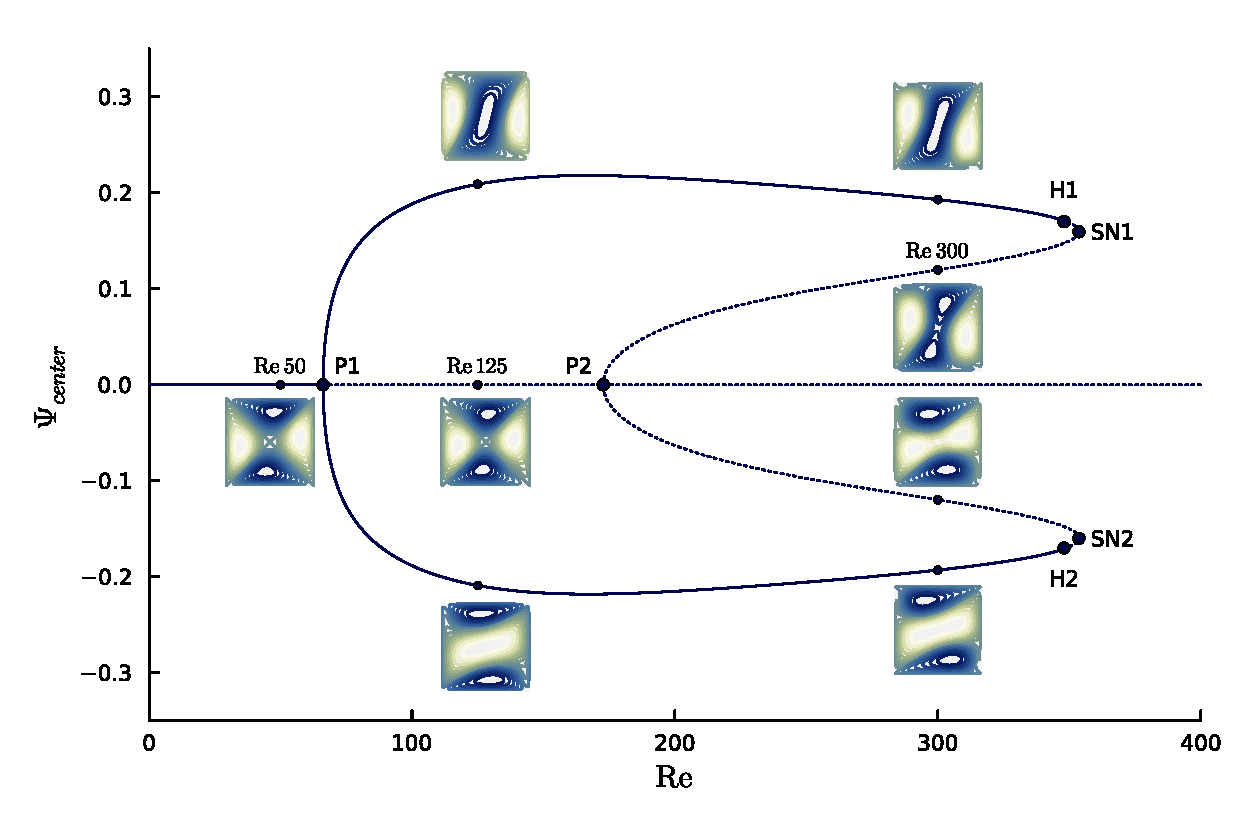
\includegraphics[width=0.9\textwidth]{figs/bifurcation_diag64x64.pdf}};
      \begin{scope}[x={(image.south east)},y={(image.north west)}]
          \draw (0.872,0.72) circle [radius=14pt];
          % \draw[->] (0.868,0.72) -- (0.9,0.72) 
          \node[anchor=south west,inner sep=0] (image) at (0.8,0.65) {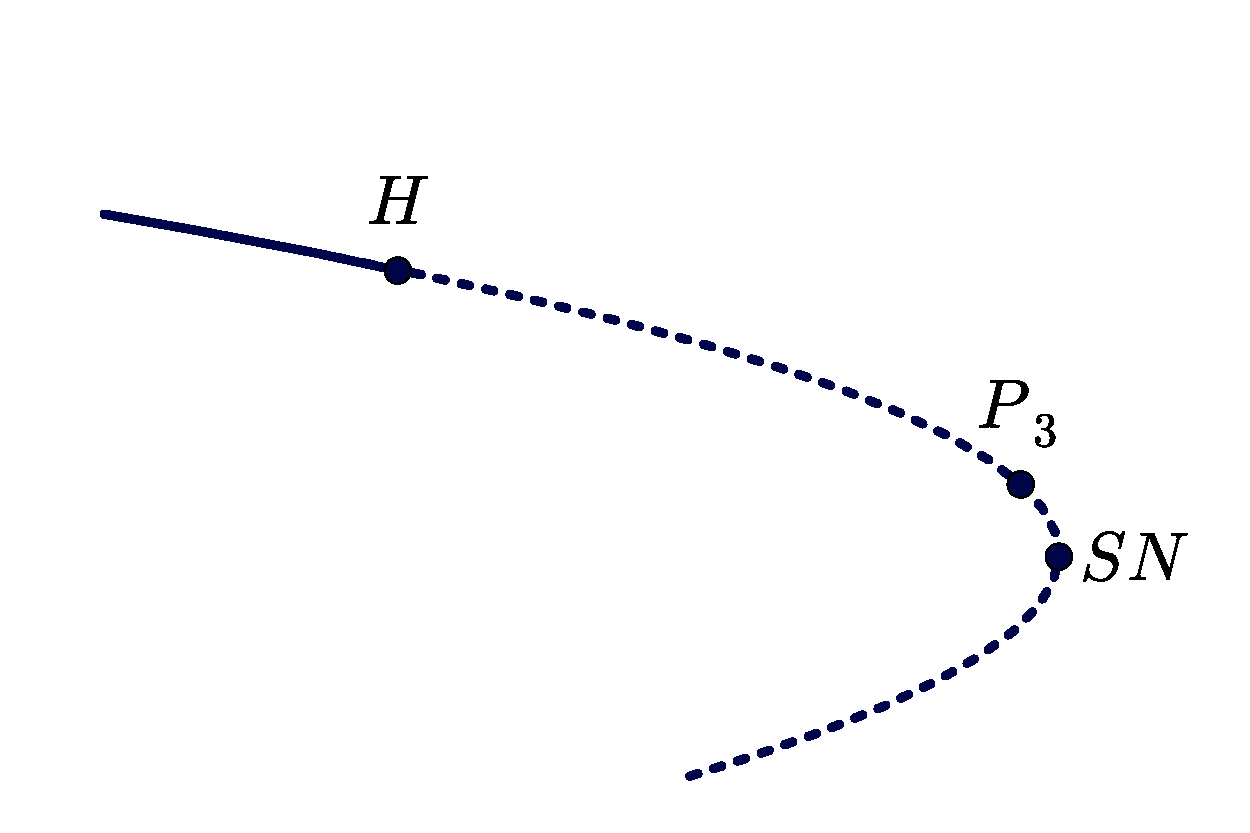
\includegraphics[width=0.3\textwidth]{figs/bifurcation_diag_zoom64x64.pdf}};
      \end{scope}
  \end{tikzpicture}
  \caption{Bifurcation diagram for the regularized version of the four-sided
    cavity flow, calculated by using the custom-developed Julia module} 
  \label{fig:bif_diag}
\end{figure}

Analyzing the new bifurcation diagram in figure \ref{fig:bif_diag} shows that
the regularized version resembles the non-regularized one regarding
bifurcations and the shape of the asymmetric branches. The reported critical
Reynolds numbers for the pitchforks $P_1$ and $P_2$ are close to those of the
original problem (scaled by $2$, see section \ref{sec:regul}). We can also see
how the regularized version converges rapidly, with only the third decimal
digits changing from a grid of size $48 \times 48$ or larger for the two
pitchforks and the saddle-node bifurcation. However, it is worth mentioning
that the pitchfork $P_2$ is not a true pitchfork as only unstable branches
(represented by the dashed line) join at this bifurcation.

On the other hand, it has been observed that the critical value for the
saddle-node in the regularized version deviates significantly from the original
value by approximately $80$ units of Reynolds. However, by increasing the
control parameter $k_0$ (fixed to $10$ in this study), the saddle-node appears
to shift further to the right. Consequently, this adjustment brings it closer
to the original bifurcation point, as it better approximates the discontinuous
step function of the boundary conditions. Nevertheless, one can not expect good
results when taking this limit as the boundary conditions are again "almost"
discontinuous.

Moreover, the Group of Nonlinear Fluid Dynamics at UPC discovered a Hopf
bifurcation ($H$) at the asymmetric branch. Furthermore, a pitchfork
bifurcation ($P_3$) was found with a critical Reynolds number close to the
saddle-node. Another branch is emerging at that location, displaying a
different asymmetric flow pattern. The following two subsections will discuss
these two bifurcation scenarios in more detail. 

\subsection{Hopf Bifurcation and Time-Periodic Flows}

The Hopf bifurcation at a critical Reynolds of around $348.3$ has not been
reported in any of the previous studies. The question that arises is if the
Hopf bifurcation is subcritical or supercritical. For the subcritical case, we
should be able to detect a stable time-periodic flow before and after the Hopf
bifurcation. After the critical value for the Hopf, all steady-solutions become
unstable, and launching a time-stepper with random values of the order of
$10^{-3}$ does reveal trajectories converging to stable periodic orbits, which
are shown in figure \ref{fig:orbit}. In order to visualize the orbit in the
phase space, the average of the vertical and horizontal velocities at the top
and left mid-points of the cavity (as defined in figure \ref{fig:cav_domain})
is used. In figure \ref{fig:orbit_bif_diag}, the amplitude of these
oscillations is shown in terms of the center value of the streamfunction and
compared to the unstable branches. Notably, the magnitudes are greater than the
expected square root growth of amplitude for unstable oscillations that
characterize a supercritical Hopf bifurcation. One can also recognize that the
stable periodic orbits pass close by the two locally attracting lower
asymmetric branches.

\begin{figure}[ht]
  \begin{subfigure}[b]{0.42\textwidth}
  \centering
  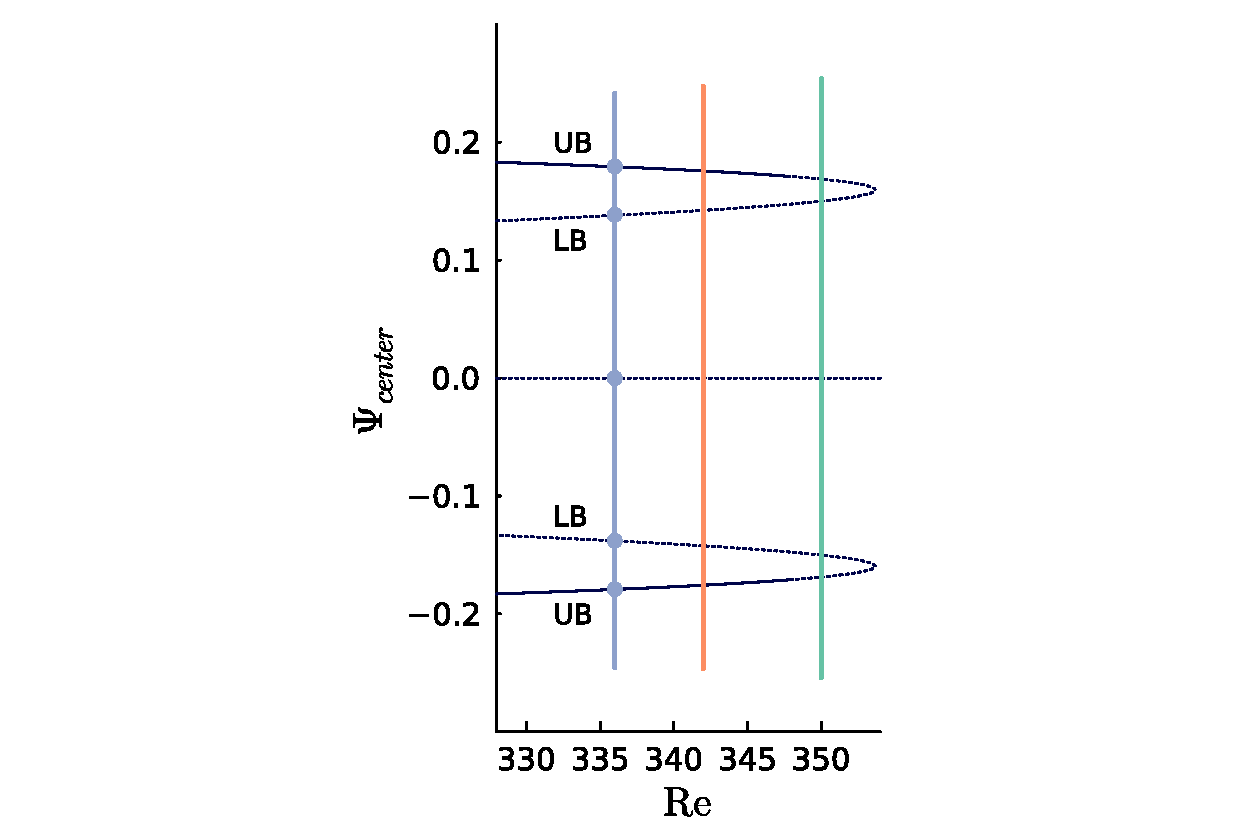
\includegraphics[trim={3cm 0 4.6cm 0},clip,width=\textwidth]{figs/orbits_bif_diag64x64.pdf}
  \end{subfigure}
  \begin{subfigure}[b]{0.58\textwidth}
  \centering
  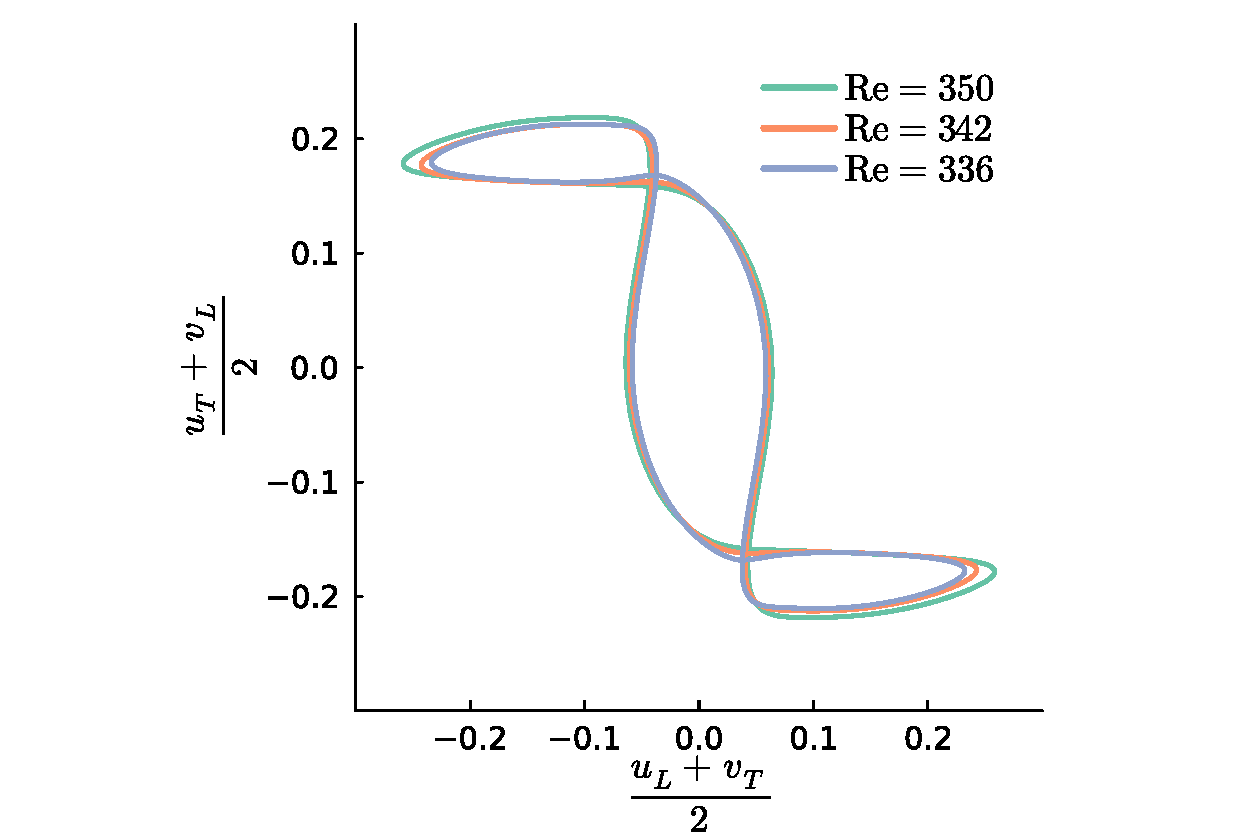
\includegraphics[trim={1cm 0cm 1cm 0cm},clip,width=\textwidth]{figs/orbits64x64.pdf}
  \end{subfigure}
  \caption{Periodic orbits at different Reynolds numbers, depicted in the
    bifurcation diagram and in a projection of phase space} 
  \label{fig:orbit_bif_diag}
\end{figure}

\begin{figure}[ht]
  \centering
  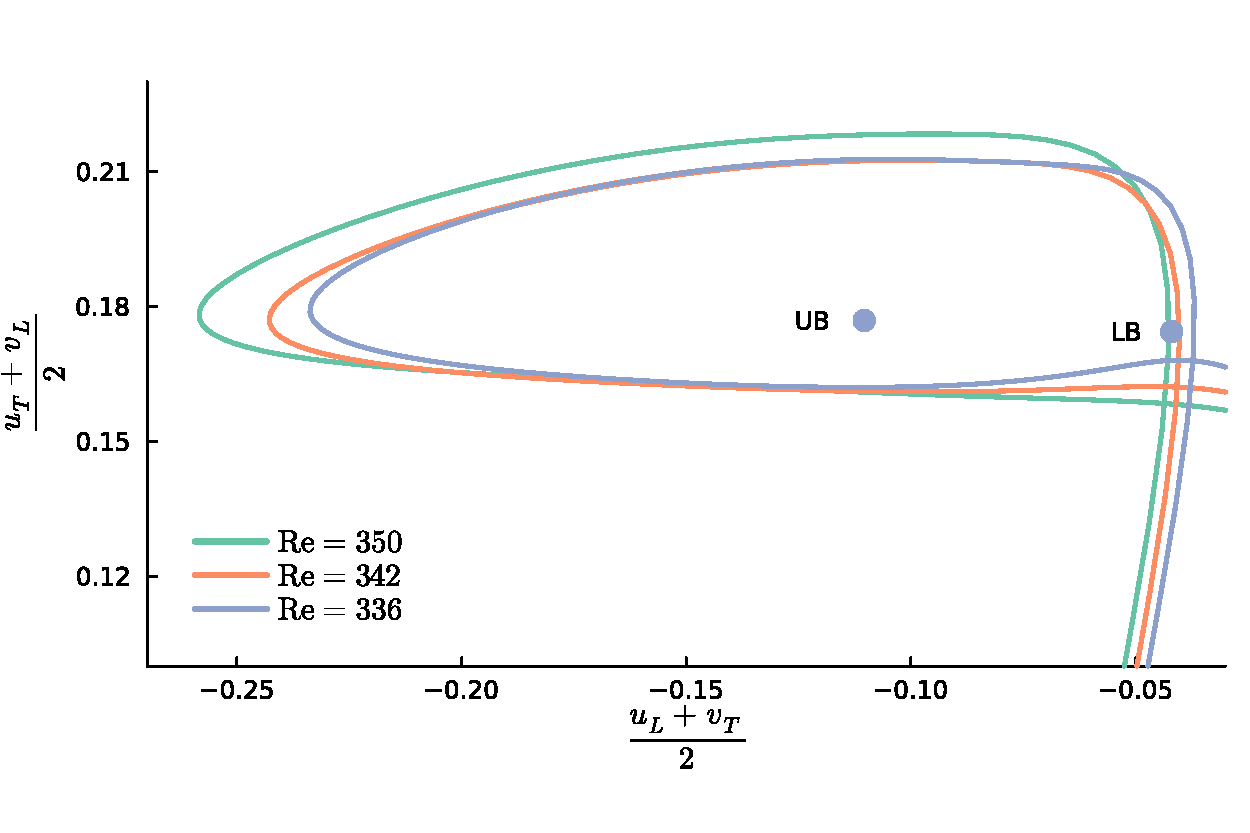
\includegraphics[width=0.8\textwidth]{figs/orbits_zoom64x64.pdf}
  \caption{Zoom of periodic orbits at different Reynolds numbers, green dots denote
  the locations of the two upper stable and unstable steady solutions}
  \label{fig:orbit}
\end{figure}
It becomes evident that stable orbits exist below the critical Reynolds number
of the Hopf bifurcation. The periodic orbits below this Reynolds number are
obtained by extracting the solutions of the $\Psi$ with the maximum amplitude
and utilizing this as initial conditions for a lower Reynolds number in the
time-stepper. These periodic orbits collapse at a Reynolds number of around
\red{335}. Time evolutions at lower values will converge to one of the stable
asymmetric branches. Additionally, unstable periodic orbits have been computed
using the MATLAB version, with the Reynolds number lower than the critical
value of the Hopf. The lower branch of these orbits connects to the lower
asymmetric branch through a homoclinic connection. Figure
\ref{fig:sub_hopf_sketch} illustrates what seems to be going on. It is still
unclear what happens in the region after the collapse of the stable larger
periodic orbits and before the homoclinic connection. Two stable solutions
coexist in this interval, namely the stable asymmetric branch and the stable
periodic orbit. From a dynamical systems point of view, these stable solutions
have to be separated by an unstable branch. This remains unclear, but this
likely corresponds to a subcritical Hopf.

\begin{figure}[h!]
\vspace{20pt}
\centering
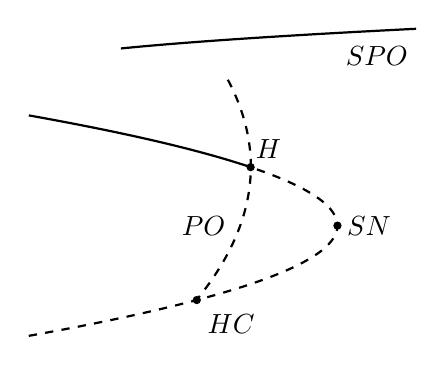
\begin{tikzpicture}[scale=0.5]
  \draw[thick, dashed] plot[smooth,domain=-2.8:1.5] ({-\x*\x},\x);
  \draw[thick] plot[smooth,domain=1.5:2.8] ({-\x*\x},\x);

  \draw[thick, dashed] plot[smooth,domain=-3.45:2.38] ({-0.12*\x*\x - 2.2},\x + 1.5);

  \draw[thick] plot[smooth,domain=0.5:1] ({10*\x*\x - 8},\x + 4);

  \fill (-1.485^2,1.485) circle [radius=3pt];
  \fill (-1.89^2,-1.89) circle [radius=3pt];
  \fill (0,0) circle [radius=3pt];

  \node at (-1.5^2 + 0.5,1.7 + 0.25) {$H$};
  \node at (-3.4,0) {$PO$};
  \node at (1,4.3) {$SPO$};
  \node at (-2.7,-2.5) {$HC$};
  \node at (0.8,0) {$SN$};
\end{tikzpicture}
\caption{Illustration of the potential subcritical Hopf, the amplitudes are
shown in the bifurcation diagram for the stable periodic ($SPO$) and the
unstable periodic orbits ($PO$) with its homoclinic connection ($HC$)} 
\label{fig:sub_hopf_sketch}
\end{figure}

\subsection{Pitchfork Bifurcation and New Asymmetric Solutions}

During the linear stability analysis conducted around the saddle-node, another
occurrence of an eigenvalue crossing and gaining a positive real part has been
identified. Figure \ref{fig:lsa} shows the three largest eigenvalues in a plot
where the Reynolds number increases and then decreases again from the
saddle-node onwards. The details of these crossings are presented in table
\ref{tab:cross}. The crossing labeled $A$ corresponds to the complex conjugate
pair associated with the Hopf bifurcation, which is denoted by $\lambda_1$ and
$\lambda_2$ in green. However, another eigenvalue crossing is found just before
the saddle-node, denoted as $B$. This second eigenvalue crossing ($\lambda_3$
in orange) lies within a range of $0.3$ in Reynolds. \\\\

\begin{minipage}[h]{\textwidth}
\begin{minipage}[b]{.4\textwidth}
\centering
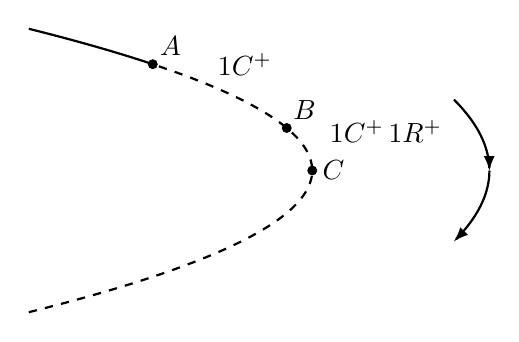
\begin{tikzpicture}[scale=0.9]
  \draw[thick, dashed] plot[smooth,domain=-2:1.5] ({-\x*\x},\x);
  \draw[thick] plot[smooth,domain=1.5:2] ({-\x*\x},\x);

  \draw[-latex, thick] plot[smooth,domain=1:0] ({2.5 + -0.5*\x*\x},\x);
  \draw[-latex, thick] plot[smooth,domain=0:-1] ({2.5 + -0.5*\x*\x},\x);

  \fill (-1.5^2,1.5) circle [radius=2pt];
  \fill (-0.6^2,0.6) circle [radius=2pt];
  \fill (0,0) circle [radius=2pt];

  \node at (-1.5^2 + 0.25,1.5 + 0.25) {$A$};
  \node at (-0.6^2 + 0.25,0.6 + 0.25) {$B$};
  \node at (0.3,0) {$C$};

  \node at (-1.5^2 + 1.3,1.6 - 0.1) {$1\mathbb{C}^{+}$};
  \node at (-0.6^2 + 1.4,0.6 - 0.05) {$1\mathbb{C}^+ \, 1\mathbb{R}^+$};
\end{tikzpicture}
\captionof{figure}{A schematic of the encountered eigenvalue crossing and 
  the direction of the linear stability analysis in figure \ref{fig:lsa}}
\label{fig:schem_saddle}
\end{minipage}\hspace{30mm}
\begin{minipage}[b]{.35\textwidth}
  \centering
  \begin{tabular}{crrr}
  \label{tab:cross}
  $n$ & $A$ ($H$) & $B$ ($P_3$) & $C$ ($SN$) \\
  \hline
  $64$ & $348.19$ & $353.356$ & $353.656$ \\
  $96$ & $348.19$ & $353.357$ & $353.654$ \\
  & & & \\
  & & & \\
\end{tabular}
\captionof{table}{Critical Reynolds numbers where crossings appear. \newline \newline}
\end{minipage}
\end{minipage}
\smallskip

\begin{figure}[h]
  \centering
  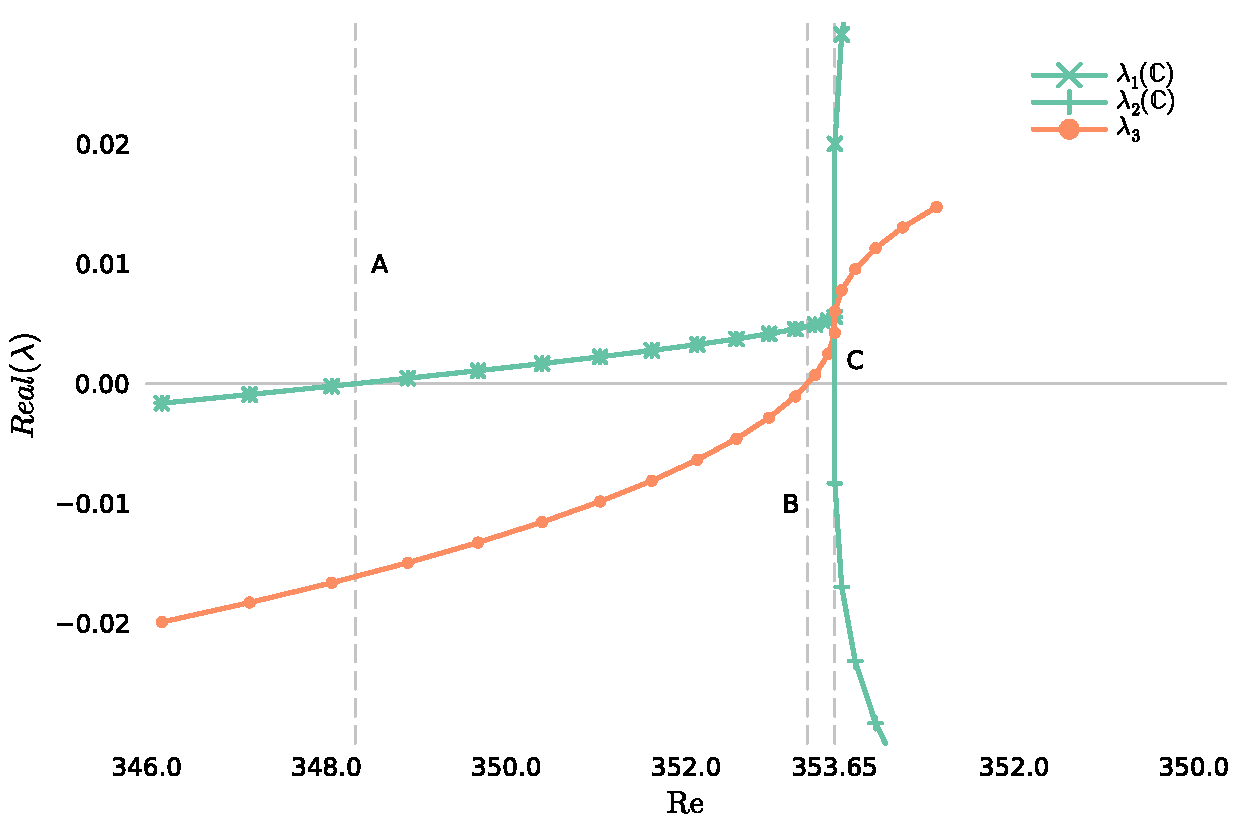
\includegraphics[width=0.8\textwidth]{figs/lsa_sn96x96.pdf}
  \caption{Linear stability analysis around saddle-node (increasing and
    decreasing Reynolds number), the real part of the three largest eigenvalues
    are shown, grid $96 \times 96$} 
  \label{fig:lsa}
\end{figure}

Additionally, close to the saddle-node, another unstable branch emerges, which
was detected by starting the natural continuation algorithm near the critical
Reynolds of the fold. This branch is depicted in figure \ref{fig:branch2} and
contains unstable solutions. The figure shows the projections onto the $\Psi$
and $u_T$ planes to distinguish the branches. One can see that for the new
branch, the center value of the streamfunction is not changing significantly,
whereas, for both the asymmetric and the second branch, there is a slight
change in the un-dimensional horizontal velocity $u_T$. Further, this branch is
connected to point $B$, corresponding to another pitchfork, denoted by $P_3$.
Linear stability analysis around the pitchfork of this new branch (figure
\ref{fig:lsa_branch2}) reveals how the eigenvalues can be related to point $B$
(i.e. $P_3$).

\begin{figure}[h!]
  \centering
  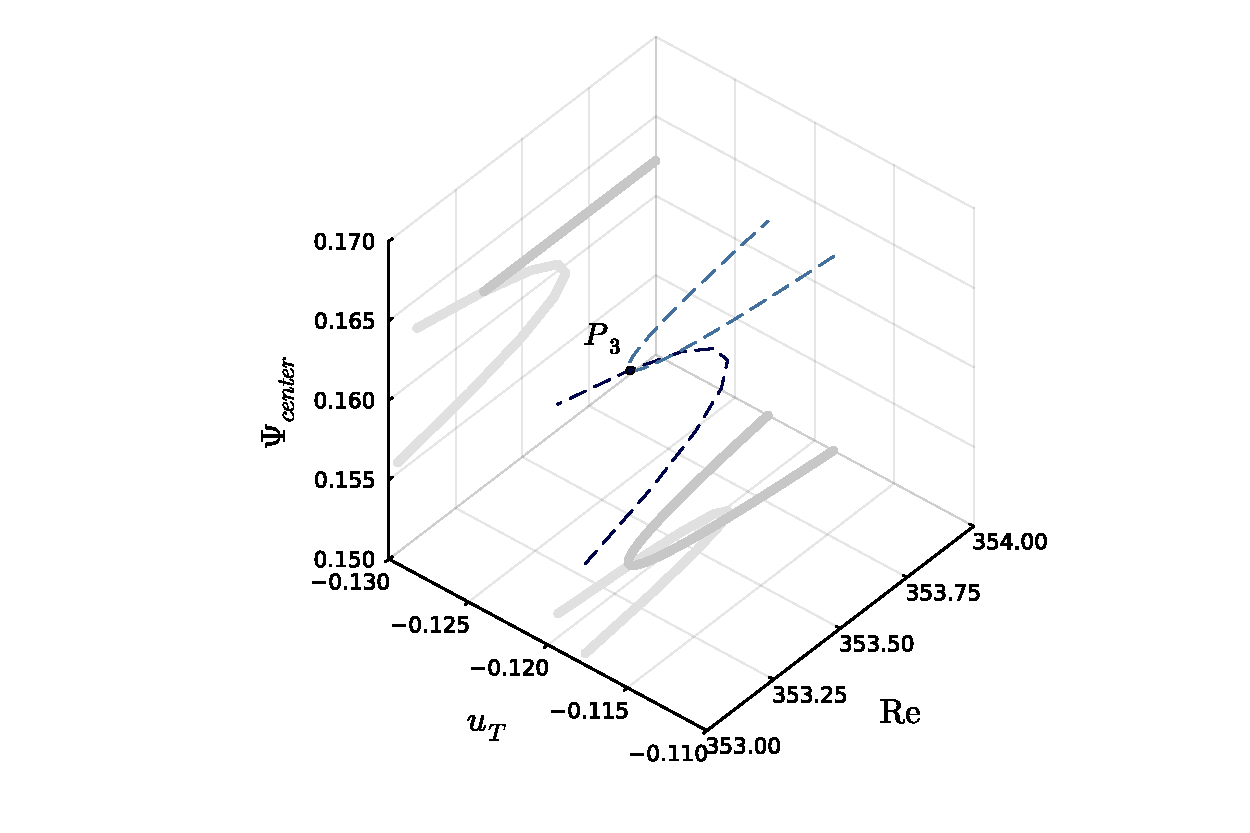
\includegraphics[width=0.8\textwidth]{figs/branch2_64x64.pdf}
  \caption{3D plot of the asymmetric branch (blue) and second branch (green) and the
    connection of the two branches at pitchfork $P_3$ ($B$)}
  \label{fig:branch2}
\end{figure}

The emergence of the second branch provides an alternative perspective on the
problem. Since we are dealing with symmetric boundary conditions, we can
observe that the streamlines of the symmetric base solution in the four-sided
lid-driven cavity flow remain unchanged under a $\pi$-rotation and \red{a point
reflection at the origin} of the cavity. The second symmetry is broken for the
two asymmetric branches, which only conserve the $\pi$-rotation symmetry.
Figure \ref{fig:sol_branch2} illustrates the two solutions of the additional
pitchfork emerging at point $B$, and it can be seen that the rotational
symmetry is no longer valid for these branches. However, both branches exhibit
the rotational symmetry to one another.

\begin{figure}[h!]
\begin{subfigure}[b]{0.33\textwidth}
  \centering
  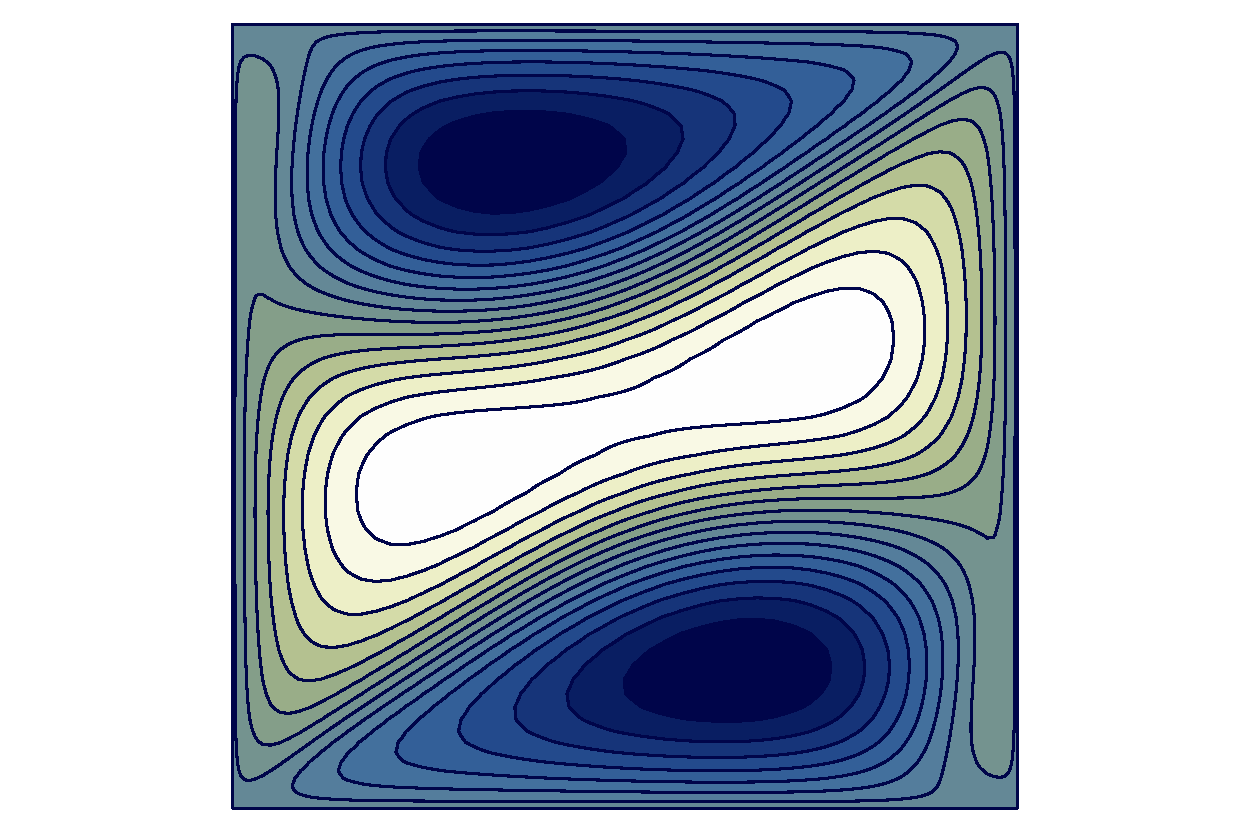
\includegraphics[trim={2cm 0 2cm 0},clip,width=\textwidth]{figs/psi_Re353.356_pf3.pdf}
\end{subfigure}
\begin{subfigure}[b]{0.33\textwidth}
  \centering
  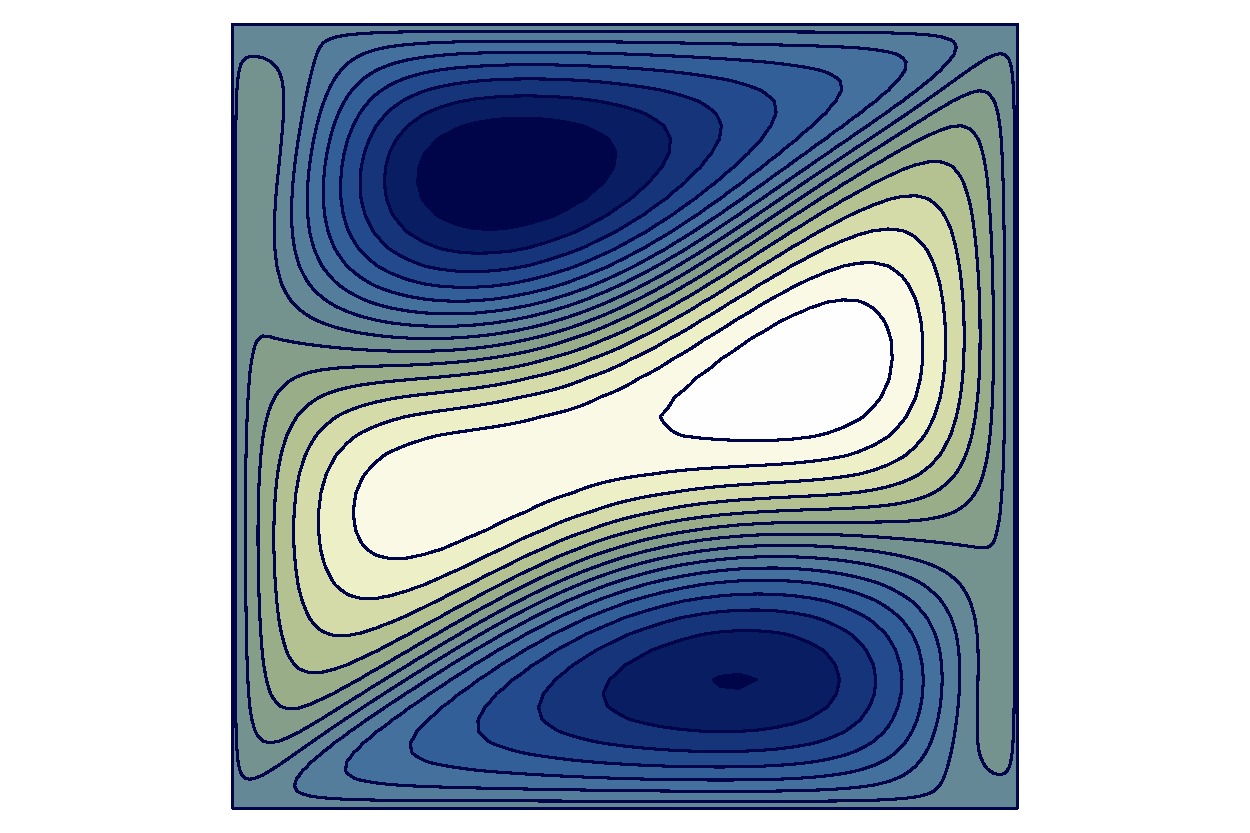
\includegraphics[trim={2cm 0 2cm 0},clip,width=\textwidth]{figs/psi_Re375.000_branch2_u_t_smaller.pdf}
\end{subfigure}
\begin{subfigure}[b]{0.33\textwidth}
  \centering
  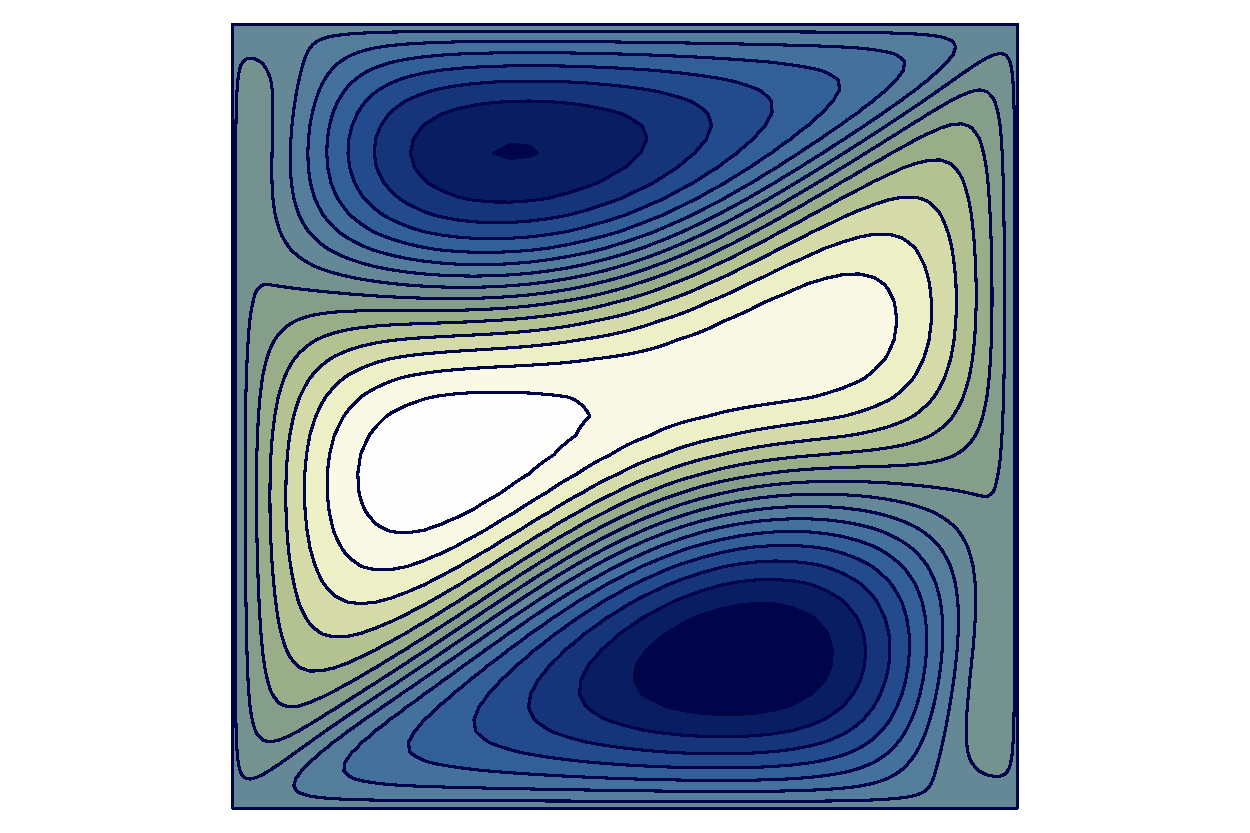
\includegraphics[trim={2cm 0 2cm 0},clip,width=\textwidth]{figs/psi_Re375.000_branch2_u_t_bigger.pdf}
\end{subfigure}
\caption{Streamlines for the pitchfork $P_3$ to the left and the two asymmetric
  solutions of the new branches to the right}
\label{fig:sol_branch2}
\end{figure}

\begin{figure}[h!]
  \centering
  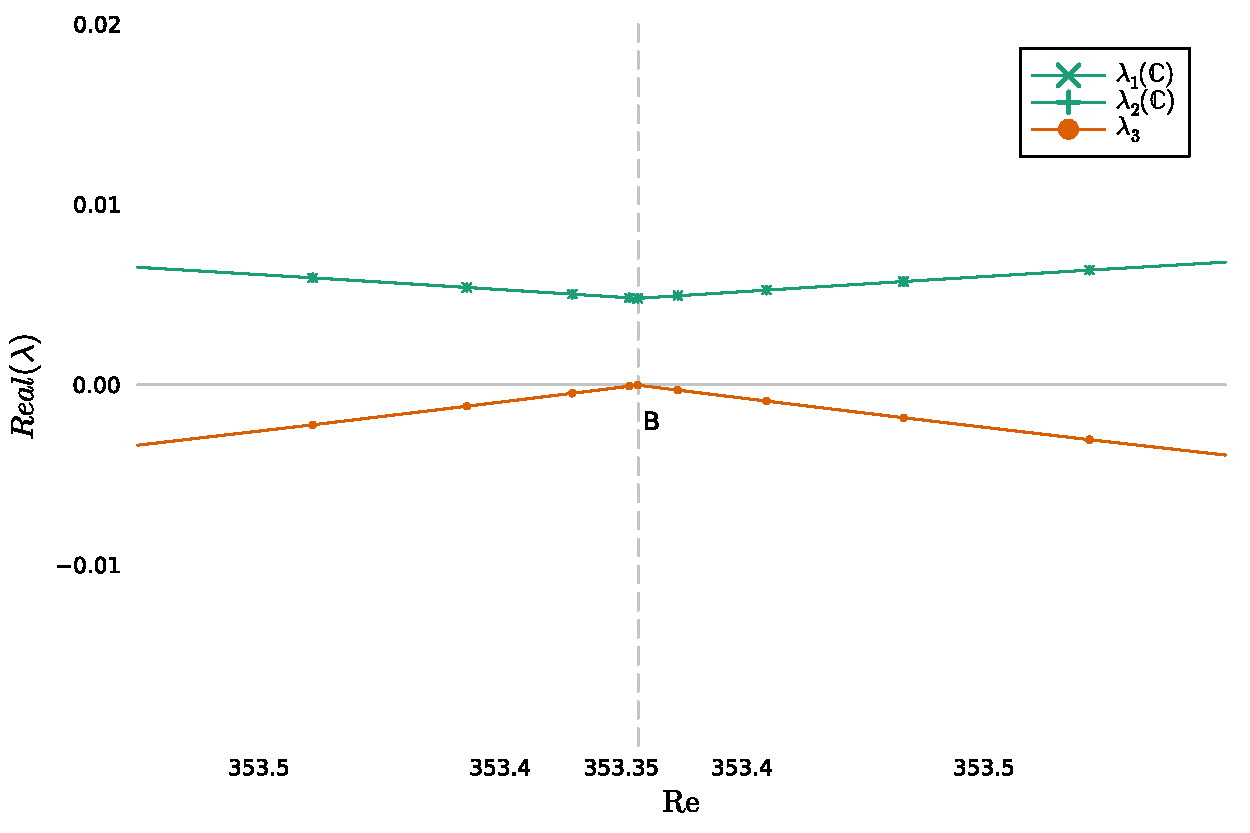
\includegraphics[width=0.7\textwidth]{figs/lsa_branch2_96x96.pdf}
  \caption{Linear stability analysis around connection $B$ of second branch
  (decreasing and then increasing Reynolds number), grid $96 \times 96$}
  \label{fig:lsa_branch2}
\end{figure}

The question that remains is what happens at the saddle-node at point $C$. The
schematic in figure \ref{fig:schem_saddle} shows the evolution of the
eigenvalues, and figure \ref{fig:lsa_zoom} shows a detail on the real part of
the eigenvalues for figure \ref{fig:lsa}. After the Hopf bifurcation ($A$), we
have a complex conjugate pair with nonzero imaginary components and a positive
real part. From pitchfork $P_3$ ($B$) onwards, the additional eigenvalue
$\lambda_3$ has a real part that also becomes positive. What happens at the
saddle-node $C$ is, first of all, that the two eigenvalues lose their imaginary
part and become purely real. Moreover, this takes place at a nonzero real part.
What seems to be happening is that one of the complex pairs (now real) "jumps"
and becomes negative. The eigenvalue configuration is depicted in the complex
plane in figure \ref{fig:complexplane} to illustrate the behavior. This
explanation is speculative because we cannot be sure that it is the eigenvalue
corresponding to the complex pair that becomes stable. It could be that two
positive eigenvalues meet at the saddle-node.

Another reason for being cautious with our interpretation is that the
saddle-node is a highly degenerated point where the Jacobian is
ill-conditioned. On top of these unreliably converged points of the Newton
solver, we are doing a linear stability analysis. Due to the degeneracy, it may
even be that the saddle-node corresponds to a double or triple zero, and
multiple eigenvalue crossings coincide. Nonetheless, these results were
obtained on a large grid for a pseudo-spectral code of size $96 \times 96$.

\vspace{100pt}

\begin{figure}[h!]
  \centering
  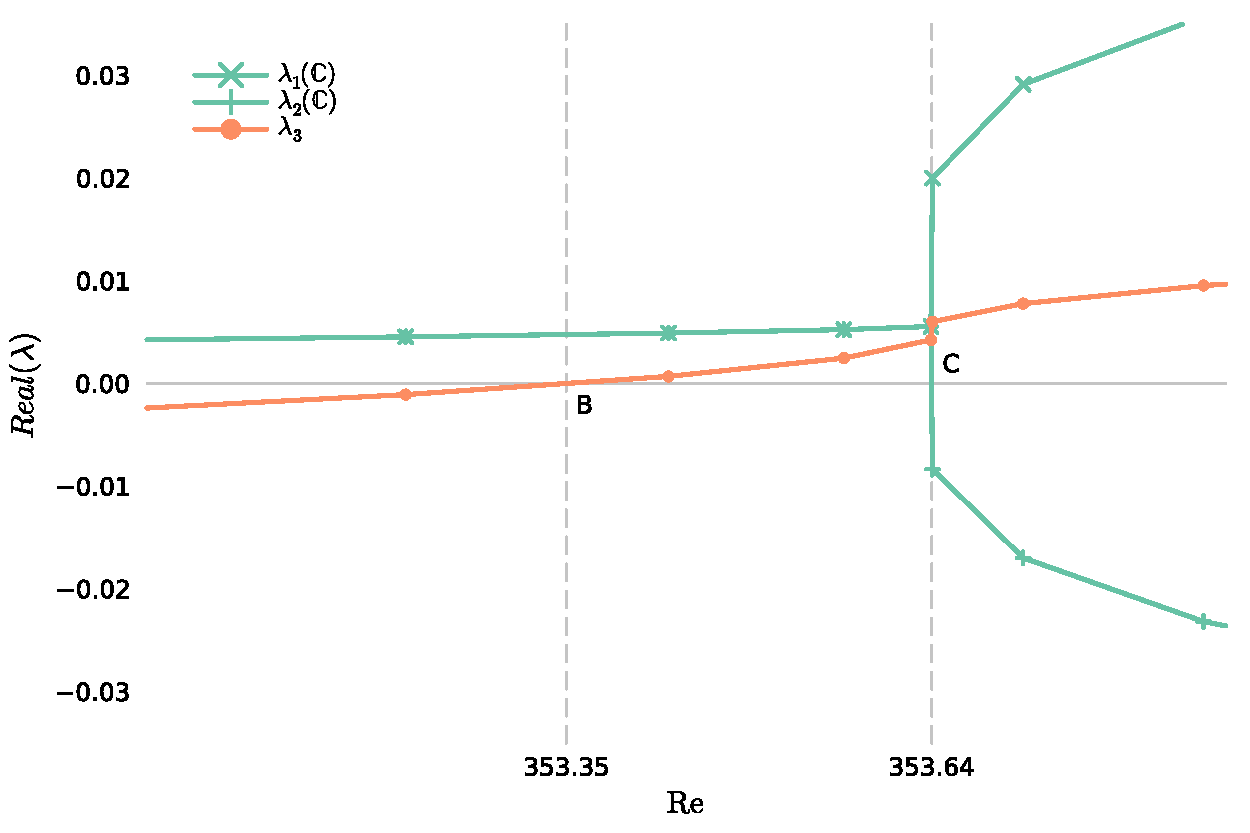
\includegraphics[width=0.6\textwidth]{figs/lsa_sn_zoom96x96.pdf}
  \caption{Zoom of figure \ref{fig:lsa} on location of saddle-node at Reynolds $353.654$} 
  \label{fig:lsa_zoom}
\end{figure}

\begin{figure}[!htbp]
\centering
\begin{subfigure}[b]{0.3\textwidth}
  \centering
  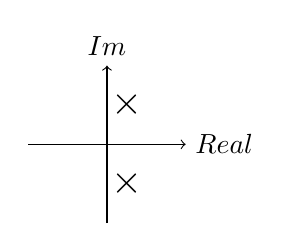
\begin{tikzpicture}
    \draw[->] (-1,0) -- (1,0) node[right] {$Real$};
    \draw[->] (0,-1) -- (0,1) node[above] {$Im$};
    \node at (0.25,0.5) {\textbf{\Large $\times$}};
    \node at (0.25,-0.5) {\textbf{\Large $\times$}};
  \end{tikzpicture}
  \caption{$1\mathbb{C}^+$, before saddle-node $C$ \newline}
\end{subfigure}
\begin{subfigure}[b]{0.3\textwidth}
  \centering
  \begin{tikzpicture}
    \draw[->] (-1,0) -- (1,0) node[right] {$Real$};
    \draw[->] (0,-1) -- (0,1) node[above] {$Im$};
    \node at (0.25,0) {\textbf{\Large $\times$}};
  \end{tikzpicture}
\caption{$2\mathbb{R}^+$, "just" before saddle-node $C$}
\end{subfigure}
\begin{subfigure}[b]{0.3\textwidth}
  \centering
  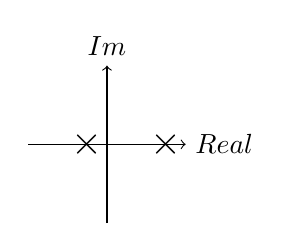
\begin{tikzpicture}
    \draw[->] (-1,0) -- (1,0) node[right] {$Real$};
    \draw[->] (0,-1) -- (0,1) node[above] {$Im$};
    \node at (0.75,0) {\textbf{\Large $\times$}};
    \node at (-0.25,0) {\textbf{\Large $\times$}};
  \end{tikzpicture}
\caption{$1\mathbb{R}^+$, at the saddle-node $C$ \newline}
\end{subfigure}
\caption{Visualization of the real and imaginary part of the complex conjugate pair
  $\lambda_1$ and $\lambda_2$ of figure \ref{fig:lsa} and \ref{fig:lsa_zoom}.}
\label{fig:complexplane}
\end{figure}
